\chapter{Problems}

% introduction
\section{Problems}

To define a problem is defining a class at the same time.

To understand a problem is to know how to check whether one solution is correct or not.
\subsection{Verifying versus Searching}


% types of problems
\section{Types of Problems}
\subsection{Computational Problems}
\subsection{Learning Problems}
\subsection{Generic Problems}

% definition and properties of techniques
\section{Techniques}
The Classification of Techniques is a core concept in daily life.
\begin{figure}
  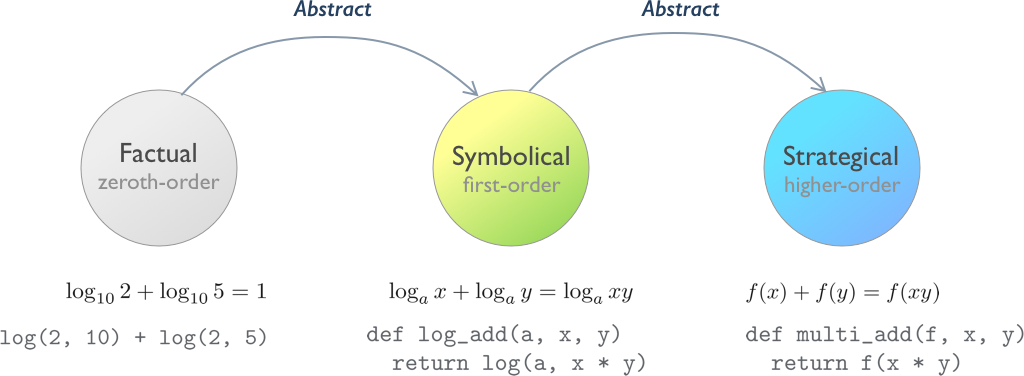
\includegraphics[width=\linewidth]{img/abstract-levels.png}
  \caption{Abstraction Levels}
  \label{fig:abstract-levels}
\end{figure}
\subsection{Robustness of Techniques}
\subsection{Frequency of Usage}
\subsection{Ad-Hoc versus Generic}
One phenominon that I experience a lot is the way people don't distinguish the difference between a ad-hoc technique and a generic technique. When a teacher or a guy present a way to solve a specific problem, few people will appreciate the robustness of this technique, that how well can you transfer your ability on this learning to another situations. But because of their inability to distinguish hardness and robustness, that leads to a dangerous place, that you have to learn too much techniques to cope with every problems, but you don't have enough time for learning these. And the teacher may think by doing an ad-hoc problem will lead to a better understanding for a more generic solving ability, which is vague. You don't learn too much on ad-hoc problems. You only know how to solve it in a nearby situations. The overall hint on a more generic solving strategies are often weak to recognize.

People don't know how to appreciate the robustness of techniques. Only can they find the dramatic changes of events. Even you simply press the button, you believe the underlining changes belongs to your smartness, well the main reason is the engineering behind the scene to smooth the user experience.
\subsection{Intensity of Signal}
\subsection{Trainability of Techniques}
Both the solving radius and the applicability.

% types of techniques
\section{Types of Techniques}
\subsection{Factual Techniques}
\subsection{Algorithmic Techniques}
\subsection{Strategic Techniques}
\subsection{Generic Techniques}
\subsection{Expansion Techniques}
